% !TEX root = ../beamer.tex
\section{Introduction}

\subsection{Cloud Manufacturing}
\begin{frame}{Brief Introduction}{Cloud Manufacturing}
\onslide<+->{Cloud manufacturing technologies includes
\begin{itemize}
\item Internet of Things
\item Cloud computing
\item Semantic Web
\item Virtualisation
\item Service-oriented technologies
\end{itemize}
}
\onslide<+->{Aims the manufacturing process to be
\begin{itemize}
\item networked
\item intelligent
\item service-oriented
\item knowledge-based
\item energy efficiency
\end{itemize}}
\end{frame}

\begin{frame}{Initial Results}{Cloud Manufacturing}
\only<1>{\begin{figure}
\centering
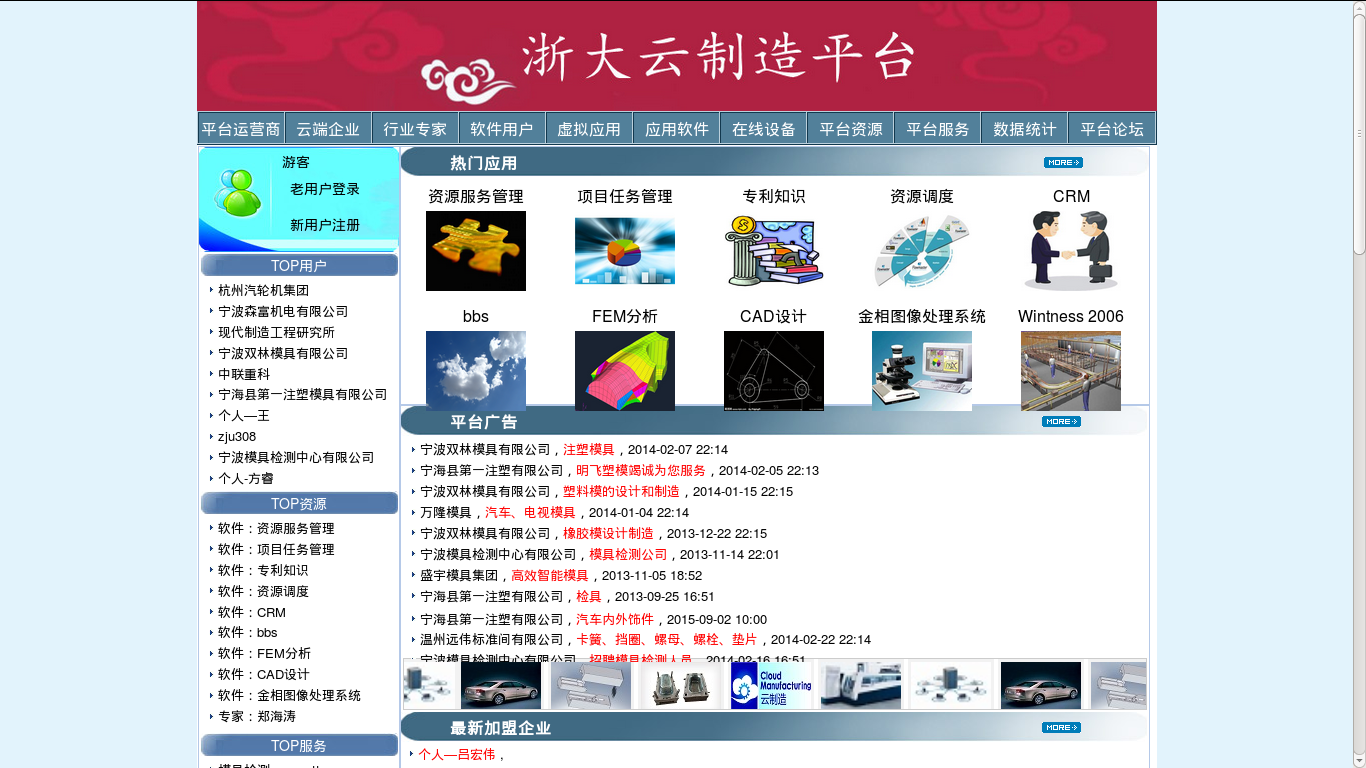
\includegraphics[width=0.95\textwidth]{figures/mainpage.png}
\caption{\href{http://mie.zju.edu.cn/cloud/}{Portal Web}}
\end{figure}}
\only<2>{
	\begin{block}{Main Component of Cloud Manufacturing prototype system}
		\begin{itemize}
			\item Platform portal system
			\item Order/Task management system
			\item Resource/Service management system
			\item Knowledg management system
			\item Commercial application sharing system
		\end{itemize}
	\end{block}
}
\end{frame}

\subsection{Current Items}

\begin{frame}{Current Items}{National High-Tech. R\&D Program, China}
\textbf{Foundation Item}: \textit{Key Technologies Research on Cloud Manufacturing Platform for Group Enterprises (No. 2015AA042101)}
\begin{block}{Main Tasks}
  \begin{itemize}
  \item Business model and standard formulating in group enterprises;
  \item Multi-tenancy technology for on-demand usage;
  \item Platform development for enterprises (Cooperate);
  \item Application demonstration (Cooperate).
  \end{itemize}
\end{block}
\end{frame}
\begin{frame}{Current Items}{National High-Tech. R\&D Program, China}
	\begin{figure}
		\centering
		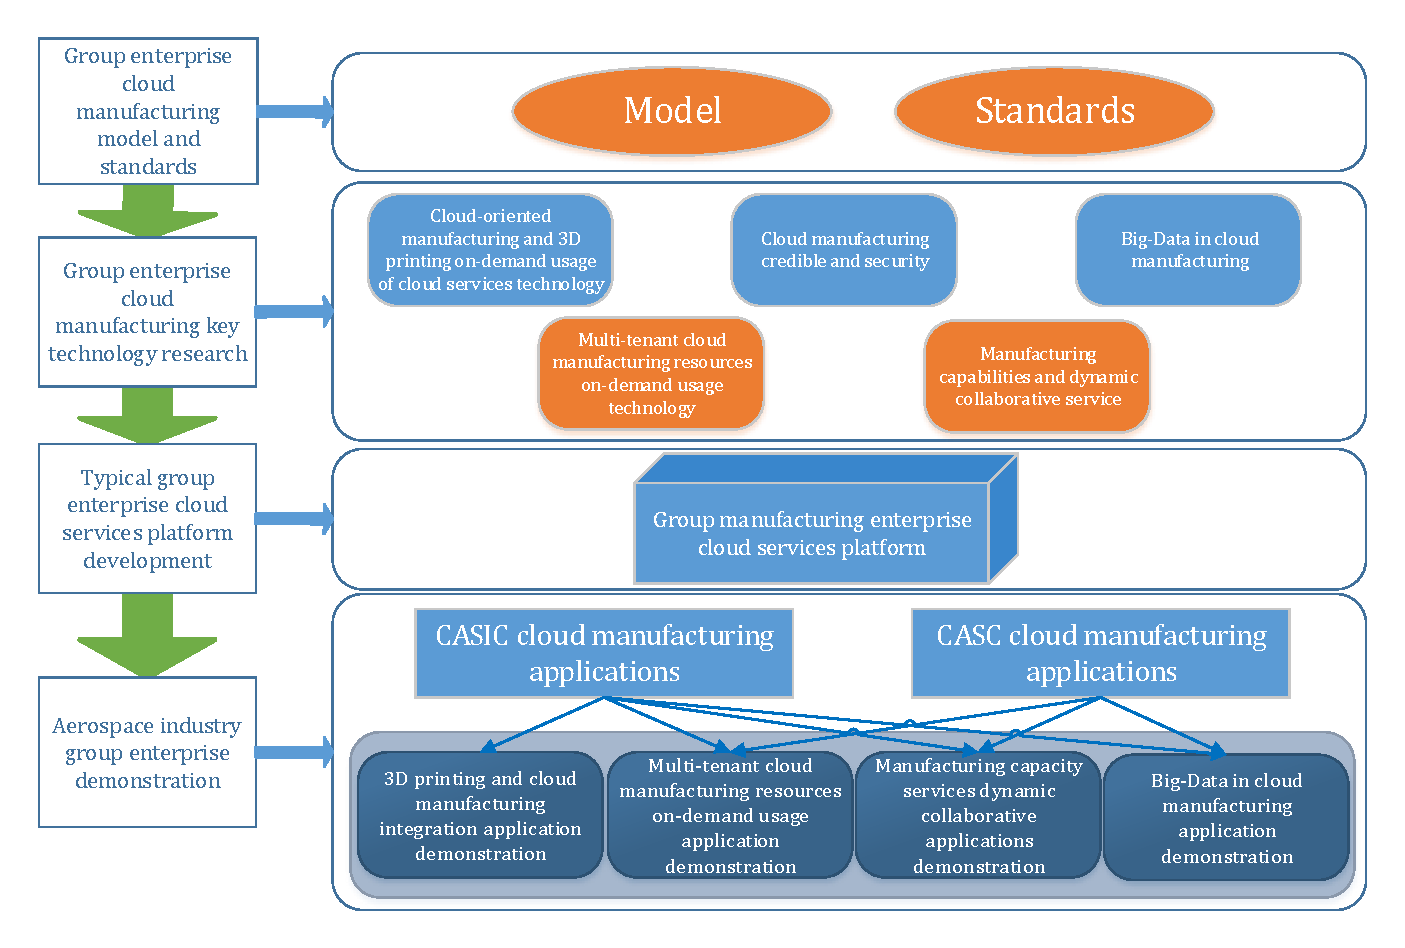
\includegraphics[height=0.85\textheight]{figures/techrouteorange.pdf}
		\caption{Technology Roadmap}
	\end{figure}
\end{frame}


\begin{frame}{Current Items}{National Natural Science Foundation, China}
\textbf{Foundation Item}: \textit{BOSS based Product Manufacturing-service Modeling and Cloud Platform Guided Service-network Evolving (No. 71571161)}
\begin{block}{Main Tasks}
\begin{itemize}
\item Methodology study for standard Manufacturing-service;
\item Methodology study for Manufacturing-service evalution;
\item Optimize the matching between services and tasks;
\item Explore the evolution of Manufacturing-service.
\end{itemize}
\end{block}
\end{frame}
\begin{frame}{Current Items}{National Natural Science Foundation, China}
	\begin{figure}
		\centering
		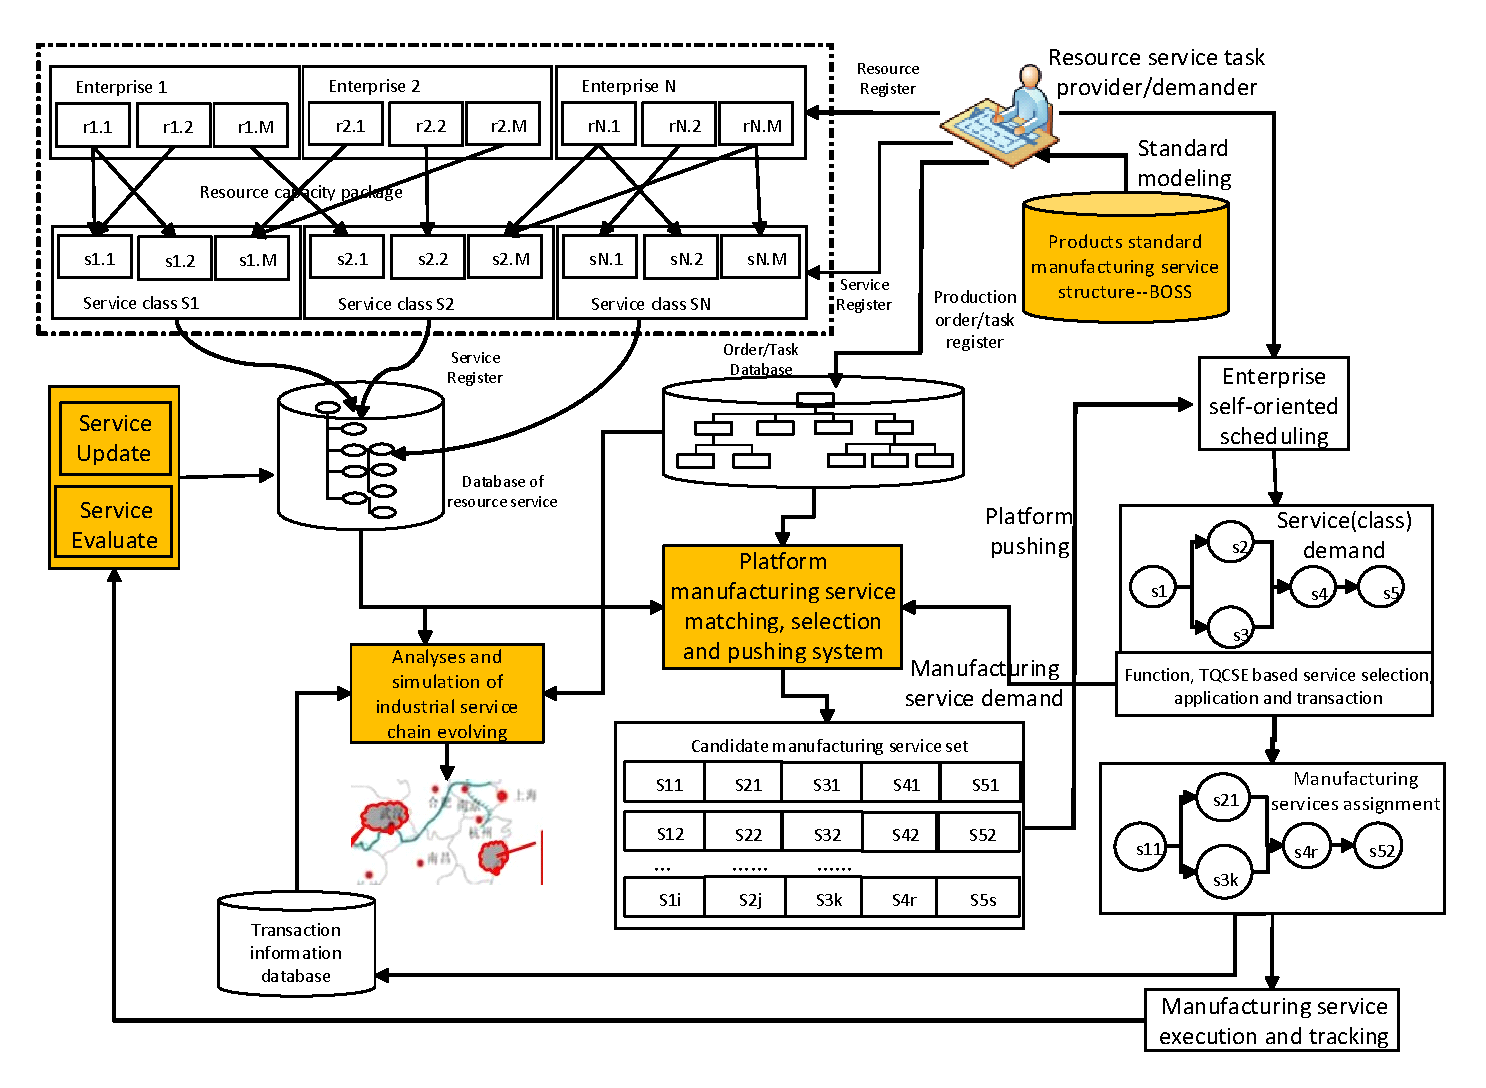
\includegraphics[height=0.85\textheight]{figures/nsf.pdf}
		\caption{Main technical research relationship map}
	\end{figure}
\end{frame}
